\section{Validation}
In this section we will validate and prove that our implementation works as expected and we will look into the performance of the implementation compared to similar alternatives.
\subsection{Benchmark}
\subsection{The JoRBA Project}
The JoRBA Project\cite{Jorba} (Jolie Rule-Based Adaptation framework) is a project about dynamic adaptation through the use of hooks and adaptation rules.

The project includes proof of concept software which is fairly large distributed system of communicating components. We downloaded the software and modified nothing but the location fields so it used our AMQP extension and our RabbitMQ message queue server as a relay for the communication between the components. We started seven components and they registered with the adaptation manager and the test client ran perfectly.

This was a great test of our request-response implementation.
\begin{figure}[H]
  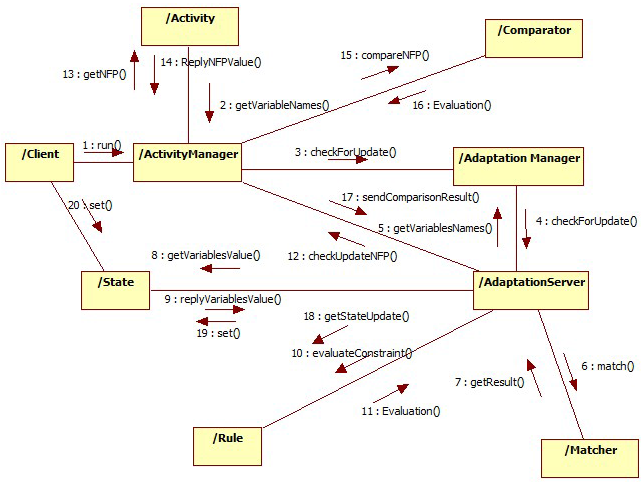
\includegraphics[width=\textwidth]{illustrations/Jorba.png}
  \caption{JoRBA collaboration diagram}
\end{figure}
\newpage